% Chapter Implementation

\chapter{Implementation}

\label{Chapter:Implementation}

This chapter explains how the existing Bazo blockchain is revised and extended. Parts of the descriptions are taken from previous papers \cite{Sgier17, Bachmann18, Blum18} and updated where necessary.

\section{Transactions}

\subsection{Stake Transaction (StakeTx)}
\label{Impl:StakeTx}

A node wishing to participate in staking can publish a stake transaction. The transaction contains the commitment key $pk_{comm}$. The StakeTx consists of the following properties:

\begin{description}
  \item[Fee] A fee that has to be paid for the validator.
  \item[Is Staking] A boolean value that indicates whether the node wants to join or leave the set of validators.
  \item[Account] The hash of the public key of the issuer.
  \item[Key Commitment] When a node wants to join the set of validators it must create a pair of public and private keys $(pk_{comm}, sk_{comm})$ using RSA. Note that this key-pair is different to the key-pair of the user's wallet. By submitting the public key $pk_{comm}$, the node commits to this key and it cannot change it in a later step. The $(pk_{comm}, sk_{comm})$ key-pair will be used in the PoS condition \ref{eq:PoSCondition}.
  \item[Signature] The signature serves the purpose of authentication. The node digitally signs the transaction with its private key $sk_{wall}$.
\end{description}

\subsection{System Parameters (ConfigTx)}

System parameters can be adjusted with this type of transaction without the need of a hard fork. The transaction must be signed by a root account in order to be accepted. Parameters to change are for example minimum staking amount, minimum waiting time, accepted time difference, slashing window size, or slashing reward.

\subsection{Funds Transaction (FundsTx)}
\label{Impl:FundsTx}

Users can transfer funds from one account to another by using a FundsTx. In fact, transferring funds is the process of subtracting an amount of coins \textit{from} the sender's account and adding the same amount of coins \textit{to} the receiver's account.

\begin{description}
  \item[Amount] The amount of Bazo coins to be transferred between accounts.
  \item[Fee] A fee that has to be paid for the validator.
  \item[Transaction Counter] The account nonce of the sender's account, prevents replay attacks.
  \item[Aggregated] Determines whether this transaction has been aggregated or not ($true/false$).
  \item[From] The public address $pk_{wall}$ of the sender.
  \item[To] The public address $pk_{wall}$ of the receiver.
  \item[Self-contained Proof] An ordered list of Merkle proofs referring back to the last epoch block to concisely prove that the sender of the transaction has enough funds to execute the transaction.
  \item[Signature] The signature serves the purpose of authentication. The node digitally signs the transaction with its private key $sk_{wall}$.
\end{description}

\subsection{Aggregation Transaction (AggTx)}

An aggregation transaction coalesces two or more $FundsTx/AggTx$. The amount that is transferred in an aggregation transaction is the sum of all $FundsTx/AggTx$. The transaction hash of an aggregation transaction is generated with a Merkle tree whose root node represents the hash of the combined hash of its children node, and the hash of its children nodes are the hash of the combined hashes of their children nodes, and so on until the leaves, where each leaf either represents the transaction hash of a $FundsTx$ or $AggTx$. Figure \ref{fig:AggTxHash} shows the Merkle tree for generating the aggregation transaction hash\label{fig:AggTxHash}, where $F$ = $FundsTx$ hash, $H[1/2]$ = intermediate hash of two $F$s, and where $A$ = $AggTx$ hash.

\begin{figure}[hbt]
\centering
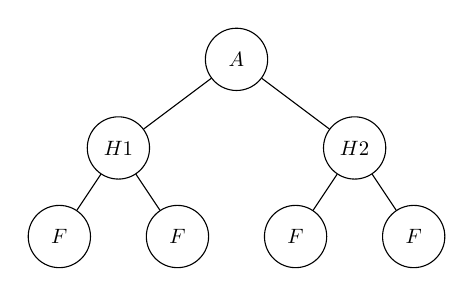
\begin{tikzpicture}[scale=0.75,node distance=20mm, 
  every node/.style={transform shape},
  level/.style={sibling distance=40mm/#1}
]

\tikzstyle{vertex}=[draw,circle,minimum size=30pt,inner sep=0pt]

\node [vertex] (r1){$A$}
  child {
    node [vertex] {$H1$}
    child {
      node [vertex] {$F$}
    }
    child {
      node [vertex] {$F$}
    }
  }
  child {
    node [vertex] {$H2$}
    child {
      node [vertex] {$F$}
    }
    child {
      node [vertex] {$F$}
    }
  };
\end{tikzpicture}  
\caption{Generating the hash of an aggregated transaction\label{fig:AggTxHash}}
\end{figure}  

\begin{description}
  \item[Hash] The transaction hash acts as a unique identifier of this aggregated transaction. The generation of the hash is shown in figure \ref{fig:AggTxHash}.
  \item[Aggregated] Determines whether this transaction has been aggregated or not ($true/false$).
  \item[Amount] The summed up value of all aggregated transaction amounts.
  \item[Transaction Counter] The value of the highest transaction counter of the aggregated transactions.
  \item[From] The public addresses $[pk_{wall}]$ of the senders.
  \item[To] The public addresses $[pk_{wall}]$ of the receivers.
  \item[Number of Transactions] The number of transactions that have been aggregated.
  \item[Hash Data FundsTxs] The hashes of all Funds Transactions (FundsTxs) included in this block in sequential order.
\end{description}

\section{Blocks}

Sharding introduces two new blocks to the system, namely epoch block and aggregation block. Multiple shardchains are running in parallel and a block of a shardchain is referred to as shard block.

Furthermore, with the introduction of transaction aggregation, validators must be able to empty blocks where all transactions have been aggregated. In that case, the pointer to the hash of a previous block would is deemed invalid. In order to keep the integrity of the blockchain, a second hash that points to the previous block without transactions is added to every block.

\begin{figure}[hbt]
\centering
\begin{subfigure}[b]{0.7\textwidth}
\centering
\begin{tikzpicture}[scale=0.8,node distance=70mm, 
  every node/.style={transform shape}
]

\tikzset{node style/.style={state,minimum width=16mm,minimum height=16mm,rectangle}}

\node[node style]              (b1){};
\node[node style, right=of b1] (b2){};

\draw[>=latex,auto=left,every loop,transform canvas={yshift=-0.25cm}]
     (b2) edge node {Previous Hash (without Tx)} (b1); 
     
\draw[>=latex,auto=left,every loop,transform canvas={yshift=0.25cm}]
     (b2) edge node {Previous Hash} (b1); 
 
\end{tikzpicture}
\caption{Before emptying a block\label{fig:DLBlockchainBefore}}
\end{subfigure}
\par\bigskip
\begin{subfigure}[b]{0.7\textwidth}
\centering
\begin{tikzpicture}[scale=0.8,node distance=70mm, 
  every node/.style={transform shape}
]

\tikzset{node style/.style={state,minimum width=16mm,minimum height=16mm,rectangle}}

\node[node style]              (b1){};
\node[node style, right=of b1] (b2){};

\draw[>=latex,auto=left,every loop,transform canvas={yshift=0cm}]
     (b2) edge node {Previous Hash (without Tx)} (b1); 
 
\end{tikzpicture}
\caption{After emptying a block\label{fig:DLBlockchainAfter}}
\end{subfigure}
\caption{Transaction aggregation results in a double-linked blockchain.}
\end{figure}

Figure \ref{fig:DLBlockchainBefore} shows two blocks where one blocks points to the previous block with two hashes. A block which only contains aggregated transactions can be emptied, resulting in an invalid previous hash. However, the second hash that points to the previous block without transactions is still valid.

\subsection{Shard Block}

A shard block is almost identical to a block introduced in Bazo before. The header of a shard block consists of the following properties:

\begin{description}
  \item[Hash] The block hash acts as a unique identifier of blocks within the blockchain.
  \item[Previous Hash] This value is equal to the identifier of the previous block in the blockchain.
  \item[Previous Hash (w/o Tx)] This value is equal to the identifier of the previous block without transactions in the blockchain. If the previous block is an epoch block, this property equals to \textbf{Previous Hash}.
  \item[Number of Bloom filter Elements] The number of elements that are in the bloom filter.
  \item[Bloomfilter] The bloom filter can be queried with $pk_{wall}$ whether the block contains a transaction of $pk_{wall}$ or not. With a false-positive rate of about 10\%, the size of the bloom filter is linearly increased or decreased to meet this target.
  \item[Number of Users In Shard] The number of users in this shard.
\end{description}

\noindent The body of a shard block consists of the following properties:

\begin{description}
  \item[Time in Seconds (Nonce)] The number of seconds that a validator needed in order to fulfill the PoS condition.
  \item[Timestamp] Refers to the block creation time (seconds elapsed since January 1, 1970 UTC).
  \item[Merkle Root] The value of the merkle tree's root node. Note that the transactions, i.e., the leaves of the Merkle tree, are ordered ascending before generating the Merkle root.
  \item[Beneficiary] The address hash of the account that receives fee payments and the block reward.
  \item[Commitment Proof] This property stores a signed message of the $Height$ that this block was created. In particular, $RSA(sk_{comm}, \text{SHA3-512}(BlockHeight))$ where $sk_{comm}$ represents the private key that corresponds to the public commitment key $pk_{comm}$ that was set in the initial StakeTx of the node. Other validators can use $pk_{comm}$ to verify the proof.
  \item[Staking Proof] The proof that the creator, i.e., the leader of this particular block is eligible to create it. This proof is similar to the self-contained proof of a FundsTx, as mentioned in Section \ref{Impl:FundsTx}.
  \item[Height] The height of a block refers to the number of previously appended blocks to the blockchain.
  \item[Shard ID] The identifier of the shard this block was created for.
  \item[Slashed Address] A validator can submit a slashing proof when appending a block, i.e., it holds the address of the misbehaving node that must be punished.
  \item[Two Conflicting Block Hashes] These two properties exhibit the block hashes where the same node has appended a block on two competing chains within the slashing window size.
  \item[Number of FundsTxs/AccTxs/ConfigTxs] Corresponds to the number of transactions of each type that are included in the block.
  \item[Hash Data FundsTxs/AccTxs/ConfigTxs] The hashes of all transactions included in this block in sequential order.
\end{description}

\subsection{Epoch Block}
\label{Impl:EpochBlock}

Opposed to shard blocks, which are created by a leader and propagated through the network to every node, epoch blocks are created non-interactively, i.e., every validator locally creates an epoch block without redistributing it based on local information. The header of an epoch block consists of the following properties:

\begin{description}
  \item[Hash] The block hash acts as a unique identifier of blocks within the blockchain.
  % \item[Previous Hash] This value is equal to the identifier of the previous block in the blockchain.
  \item[Previous Hashes] This value is equal to the identifier of the previous blocks of every shard.
  % \item[Previous Hash (w/o Tx)] This value is equal to the identifier of the previous block without transactions in the blockchain.
  \item[Previous Hashes (w/o Tx)] This value is equal to the identifier of the previous blocks of every shard without transactions.
\end{description}

\noindent The body of an epoch block consists of the following properties:

\begin{description}
  \item[Timestamp] Refers to the block creation time (seconds elapsed since January 1, 1970 UTC).
  \item[Merkle Root] The value of the Merkle tree's root node.
  \item[Height] The height of a block refers to the number of previously appended blocks to the blockchain plus one.
  \end{description}

\subsection{Aggregation Block}

An aggregation block contains aggregated transactions of a particular shard and is created by a validator with the role \textit{Aggregator}. An aggregation block for shard $s$ can only created by a validator of shard $s$. Furthermore, an aggregation block at block height $h$ serves as a proposal to a leader at block height $h + 1$. The header of an aggregation block consists of the following properties:

\begin{description}
  \item[Hash] The block hash acts as a unique identifier of blocks within the blockchain.
  \item[Previous Hash] This value is equal to the identifier of the previous block in the blockchain.
  \item[Previous Hash (w/o Tx)] This value is equal to the identifier of the previous block without Transactions in the blockchain.
  \item[Number of Bloom filter Elements] The number of elements that are in the bloom filter.
  \item[Bloom filter] The bloom filter can be queried with $pk_{wall}$ whether the block contains a transaction of $pk_{wall}$ or not. With a false-positive rate of about 10\%, the size of the bloom filter is linearly increased or decreased to meet this target.
\end{description}

\noindent The body of a shard block consists of the following properties:

\begin{description}
  \item[Time in Seconds (Nonce)] The number of seconds that a validator needed in order to fulfill the PoS condition.
  \item[Timestamp] Refers to the block creation time (seconds elapsed since January 1, 1970 UTC).
  \item[Merkle Root] The value of the merkle tree's root node. Note that the transactions, i.e., the leaves of the Merkle tree, are ordered ascending before generating the Merkle root.
  \item[Beneficiary] The address hash of the account that receives fee payments and the block reward.
  \item[Commitment Proof] This property stores a signed message of the $Height$ that this block was created. In particular, $RSA(sk_{comm}, \text{SHA3-512}(BlockHeight))$ where $sk_{comm}$ represents the private key that corresponds to the public commitment key $pk_{comm}$ that was set in the initial StakeTx of the node. Other validators can use $pk_{comm}$ to verify the proof.
  \item[Staking Proof] The proof that the creator, i.e., the leader of this particular block is eligible to create it. This proof is similar to the self-contained proof of a FundsTx, as mentioned in Section \ref{Impl:FundsTx}.
  \item[Height] The height of a block refers to the number of previously appended blocks to the blockchain.
  \item[Shard ID] The identifier of the shard this block was created for.
  \item[Number of AggTxs] Corresponds to the number of aggregation transactions that are included in the block.
  \item[Hash Data AggTxs] The hashes of all transactions included in this block in sequential order.
\end{description}
